% Principal Component Analysis
\section{Principal Component Analysis (PCA)}
\label{sec:pca}

Principal Component Analysis (PCA) is a decomposition of data into linearly uncorrelated components, ordered by their explained variance. It turns out that these axes are the right-singular eigenvectors $\mathbf{V}$ that are found from SVD. SVD and PCA have correspondence (cf. section \ref{sec:pcasvd}). My guess is that the advantage of PCA is that its results are interpretable in terms of commonly used summary statistics of the distribution (namely the variances or Pearson correlations of the data).
\\

More elaborately, for a data matrix $\mathbf{X}\in\mathbb{R}^{N\times p}$, PCA extracts the ordered, rank-$p$, orthonormal basis in which the $p\times p$ covariance matrix of $\mathbf{X}$ is diagonal. The basis vectors are called the principal axes or principal directions of the data, and their ordering is by the magnitude of the variance that they explain. 
\\

The property that the covariance matrix is diagonal in the principal component basis means that projecting the data onto any of the basis vectors extracts a linearly uncorrelated component of the data that has variance corresponding to the corresponding eigenvalue of the covariance matrix.
\\

Just like with SVD, the ordering of the principal component basis in terms of their explained variance allows for lower-rank approximations of the data matrix to be constructed (section \ref{sec:svd}). Just like SVD, the lower rank approximations $\mathbf{X}$ are the best possible approximations with respect to the Frobenius Norm (cf. section \ref{sec:frobenius}). 
\\

The $p\times p$ covariance matrix  $\mathbf{C}$ of $\mathbf{X}$ is:

\begin{equation}
\mathbf{C} = \frac{\left(\mathbf{X}-\left<\mathbf{X}\right>\right)^T\left(\mathbf{X}-\left< \mathbf{X}\right>\right)}{n-1}
\end{equation}

Where $\left(\mathbf{X}-\left<\mathbf{X}\right>\right)^T$ is often referred to as the \textit{centered} data matrix. The covariance matrix is a symmetric, positive-definite matrix that can be diagonalized with orthonormal eigenvectors $\mathbf{V}$ and positive (or vanishing) eigenvalues $\lambda_i$:

\begin{equation}
\mathbf{C} = \mathbf{V}\mathbf{\Lambda}\mathbf{V}^T
\end{equation}

Where the eigenvectors in $V$ are ordered so that the eigenvectors along the diagonal of $\mathbf{\Lambda}$ have decreasing magnitude. The eigenvectors are the principal axes or principal directions of the data.


% Relationship between PCA and SVD
\subsection{Relationship between PCA and SVD}
\label{sec:pcasvd}
This is based on a great Stack Exchange answer \cite{amoeba2015svdpca}.

Let the singular value decomposition of the centered data matrix be:

\begin{equation}
\left(\mathbf{X}-\left<\mathbf{X}\right>\right) = \mathbf{U}\mathbf{\Sigma}\mathbf{V}^T
\end{equation}

Then:

\begin{equation}
\mathbf{C} = \frac{\mathbf{V\Sigma U}^T\mathbf{U\Sigma V}^T}{n-1} = \mathbf{V}\frac{\Sigma^2}{n-1}\mathbf{V}^T
\end{equation}

That means that:

\begin{itemize}
\item The principal axes are the right-singular vectors $\mathbf{V}$ that are obtained during SVD.
\item The singular values and the eigenvalues of the covariance matrix are related via $\lambda_i = \frac{\sigma_i^2}{n-1}$.
\end{itemize}



\subsection{Tracking Principal Components over Time}
Given the direct parallel between PCA and SVD, the identical issue with sign flips emerges with the principal component basis, and the remedy is the same. See section \ref{sec:svd_tracking}.


\subsection{$L^1$-Norm Principal Component Analysis ($L^1$ PCA)}
\label{sec:l1pca}

L1-Norm Principal Component Analysis is an alternative to conventional PCA that provides better robustness to outliers. Exact solutions exist in polynomial time, as well as more efficient approximate methods. \citeasnoun{brooks2014pure} establishes that the PCA under $L^1$ norm is found by successive fitting of hyperplanes under $L^1$ error in progressively smaller subspaces. Much like the $L^2$ distance of a point to a hyperplane is given by the radius of a circle around that point, the $L^1$ distance of a point to a hyperplane is given by its intersection of a rhombus. This has the (kind of quirky) consequence that the distance of all points to a hyperplane is always measured directly along one of the coordinate axes (and it is the same coordinate axes for each of the points). This, in turn, implies, that in some subspace $\mathbb{R}^m$, the $L^1$ best-fit hyperplane can be found by performing an $L^1$ regression with each of the $m$ dimensions serving as the explanatory variable, and then selecting the regression result that had the smallest residual.

\begin{figure}
\centering
    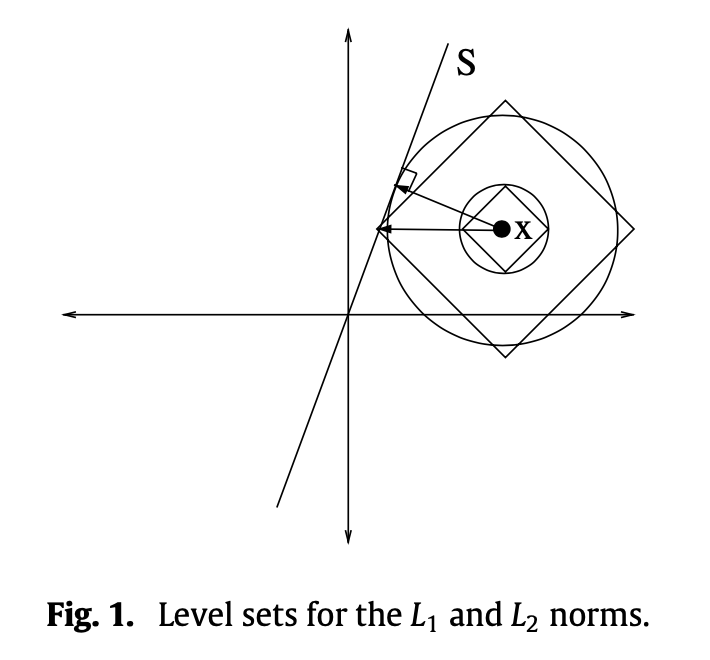
\includegraphics[width=0.4\textwidth]{l1pca.png}
    \caption{Distance of a point to a hyperplane in $L^1$ and $L^2$. The $L^1$ distance in this case is just the distance along the $x$ axis. If the hyperplane was cutting a shallower angle, then the distance would be measured along the $y$ axis. The best fit hyperplane to many points in $\mathbb{R}^2$ would be found by regressing the data points once with $y = \beta x + \epsilon$ and once with $x = \beta y + \epsilon$ and selecting the result with the smaller $||\epsilon||_1$. (The figure is from J. P. Brooks (2014).}
    \label{fig:l1pca}
\end{figure}


\subsubsection{Example: Netflix Prize, Matrix Completion}
